\chapter{Introduction}
\label{chap:Intro}


\section{Ultrafast Science}

Since the discovery of the laser \cite{schawlowInfraredOpticalMasers1958, maimanStimulatedOpticalRadiation1960} and the subsequent demonstration of nonlinear optics \cite{frankenGenerationOpticalHarmonics1961, armstrongInteractionsLightWaves1962}, one of the areas that has seen a great amount of interest is the use of lasers to study the dynamics of various systems.  This is generally done by taking advantage of the ability to create a pulsed laser \cite{demariaPicosecondLaserPulses1971}.  This occurs when the spectral phase and amplitude of a laser coherently combines to create an intense burst of light as a function of time.  As an example, a typical approximation is to assume that the electric field $\mathcal{E}(t)$ of a laser pulse can be written as a Gaussian, such as
\begin{equation}
	\label{eqn:gaussian_pulse}
	\mathcal{E}(t) = \mathcal{E}_0 e^{-2\ln 2(\frac{t}{\Delta t})^2}\cos(\omega_0 t + \theta(t))
\end{equation}
where $\Delta t$ is the pulse duration, $\omega_0$ is the carrier frequency, and $\theta(t)$ determines the temporal relationship between the frequency components that are within the pulse bandwidth.  An example of just such a pulse shape is shown in figure \ref{fig:gaussian_pulse} in both time and frequency, and it can be shown that the pulse duration $\Delta t$ is inversely proportional to the spectral bandwidth $\Delta\omega$.  This entails that larger bandwidths are required to achieve shorter transform limited pulse durations.

\begin{figure}
	\centering
	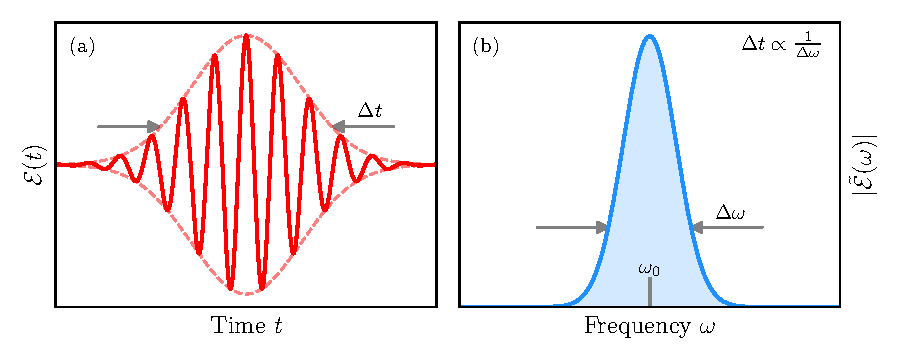
\includegraphics[width=1.0\textwidth]{figures/Introduction/gaussian_pulse.pdf}
	\caption[Example of a typical Gaussian pulse in time and frequency]{Example of a typical Gaussian pulse in time (a) and frequency (b).  The pulse duration $\Delta t$ and the spectral bandwidth $\Delta\omega$ are shown, as well as the relationship between them.}
	\label{fig:gaussian_pulse}
\end{figure}

The evolution of pulse duration since the 1960s is highlighted in figure \ref{fig:Pulse_duration}, and it can be seen that there has been a tremendous push by the community to produce ever shorter pulses.  The need for ever shorter pulse durations is rooted in how dynamics can be extracted from a system using pulsed lasers, and this is typically done through what is known as a pump/probe experiment. A schematic of a pump/probe experiment is shown in figure \ref{fig:pump_probe}.  The core concept revolves around the use of one laser pulse to induce a change within a physical system and a second laser pulse to probe the perturbed system at a variable time later, known as the time delay $\tau$.  Each of these time delays can be thought of as a single film frame, and by varying the time delay, one can construct a movie of the dynamics induced by the pump pulse.  

\begin{figure}
	\centering
	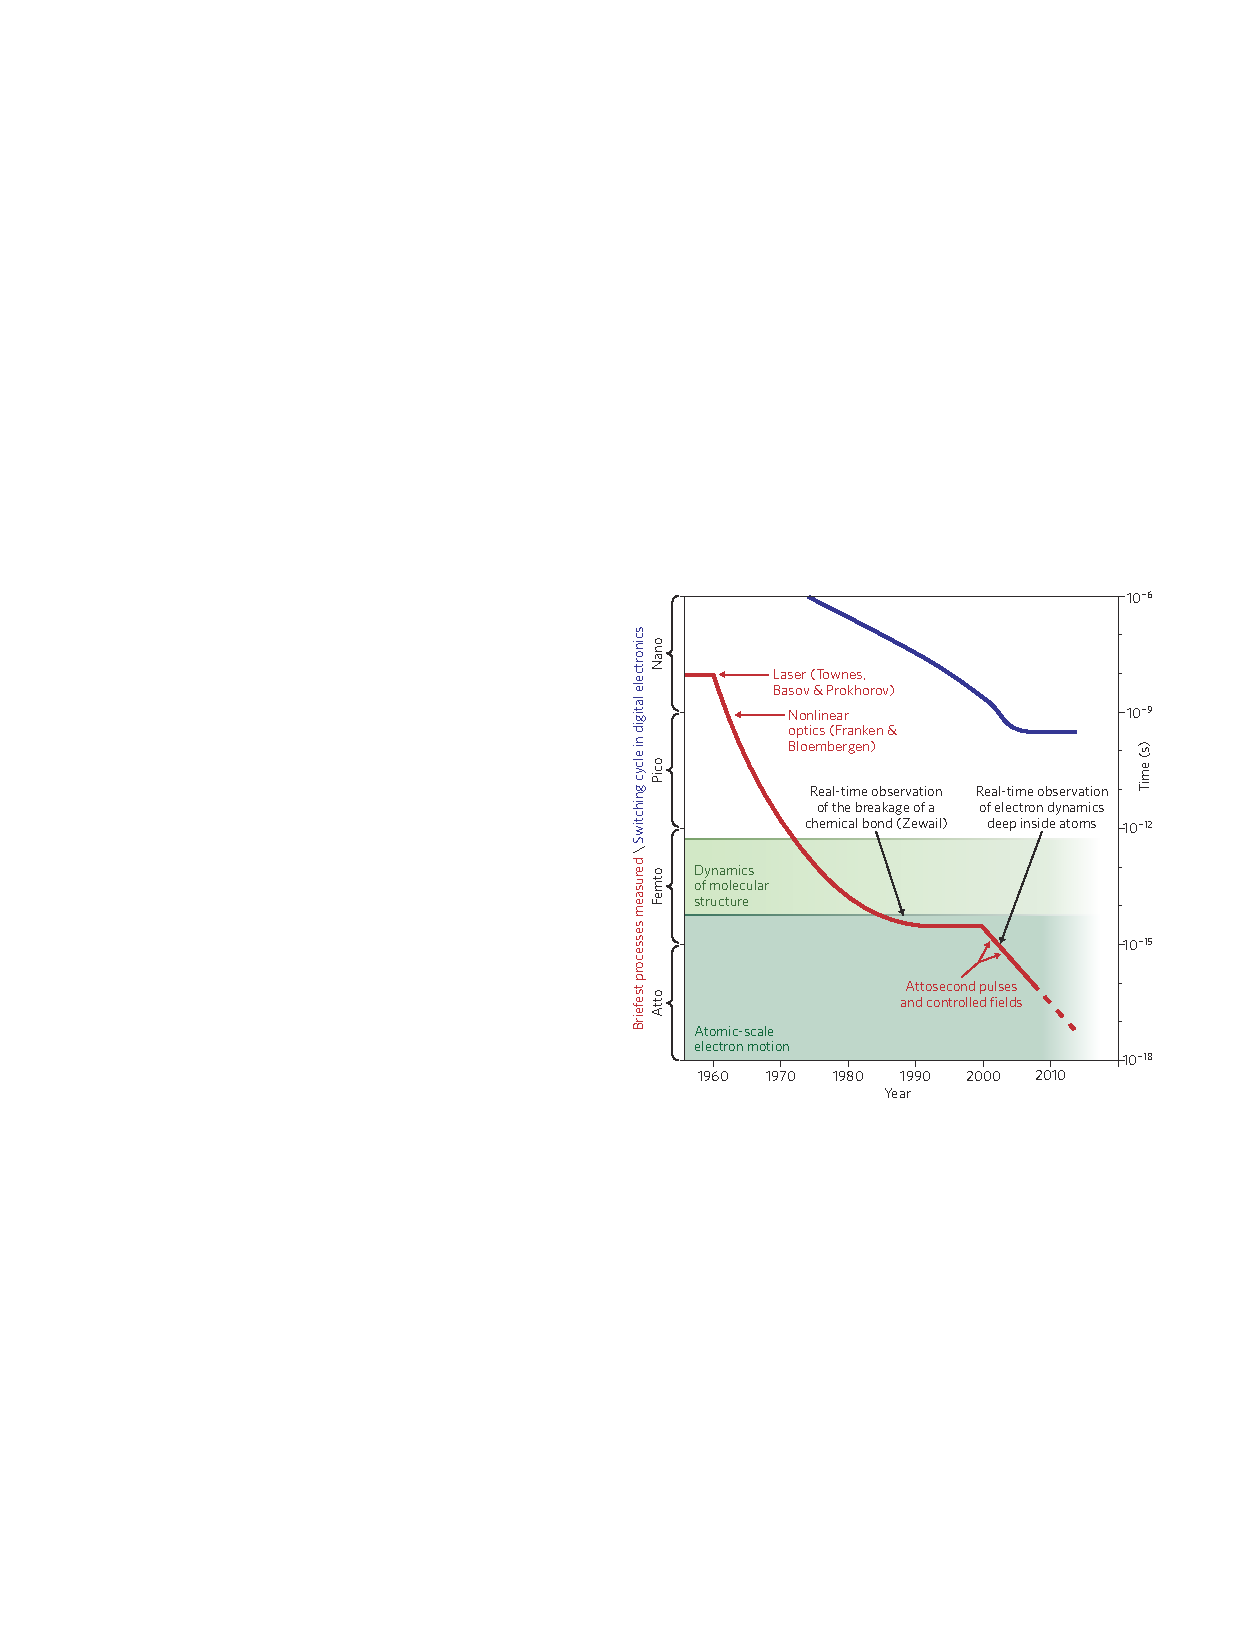
\includegraphics[width=0.5\textwidth]{figures/Introduction/Pulse_duration.pdf}
	\caption[Pulse duration as a function of time since the 1960s]{Pulse duration as a function of time since the discovery of the laser in 1960.  Adapted from \cite{krauszAttosecondMetrologyElectron2014}.}
	\label{fig:Pulse_duration}
\end{figure}

The temporal resolution of this ``movie'' is ultimately limited by the pulse duration of both the pump and probe because time is not an observable in these experiments and it can only be deduced by varying the delay.  Thus, to access processes that happen on a short timescale you need a pulse with an even shorter pulse duration.  The types of processes that are unlocked as the pulse duration get shorter and shorter is shown in figure \ref{fig:Pulse_duration}.  Once the pulses are in the femtosecond ($10^{-15}$ s) regime, then the dynamics of molecular structure and motion can be observed in real-time, and the experimental demonstration of this was awarded the Nobel Prize in 1999 \cite{zewailLaserFemtochemistry1988}.  To go beyond this regime to study the dynamics of electrons on their natural time scale, then one needs to have attosecond ($10^{-18}$ s) pulses.  The breakthrough that enabled such pulses to be generate is high-harmonic generation, and it will be discussed in the next section.

\begin{figure}
	\centering
	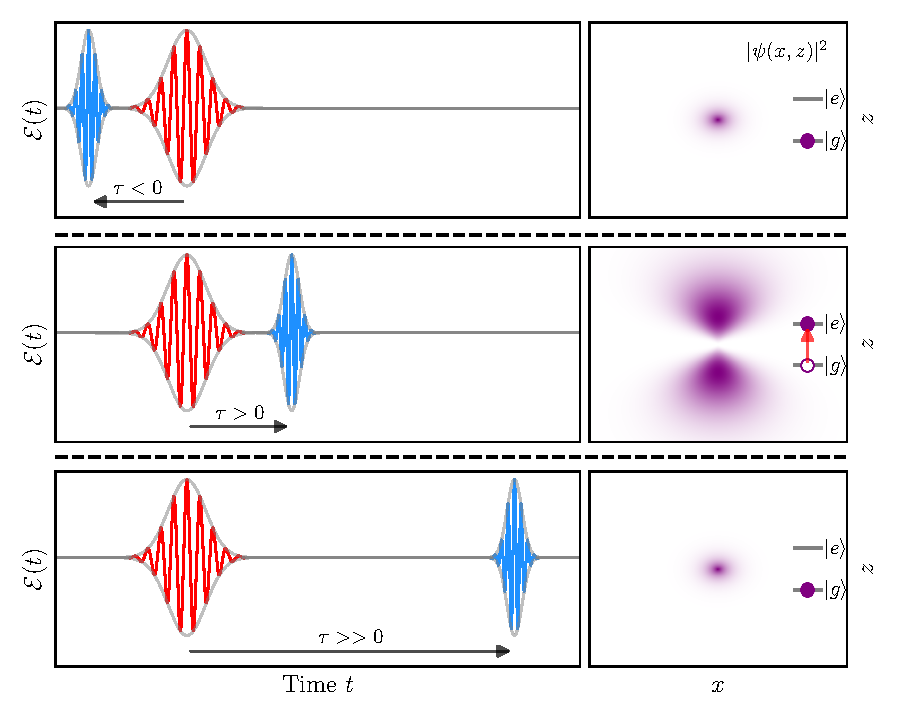
\includegraphics[width=0.9\textwidth]{figures/Introduction/pump_probe.pdf}
	\caption[Schematic of as pump/probe experiment]{Schematic of a pump/probe experiment as a series of frames constituting a movie.  Each frame is given by a different time delay between the pump (red pulse) and the probe (blue pulse).  In this simple example an electron in a hyrdogenic atom is excited from the ground state $\ket{g}$ to an excited state $\ket{e}$ that has some finite lifetime.  The state of the atom that the probe pulse observes is shown in the panels of the right.  If the probe pulse arise before the pump, then the ground state is observed.  If the probe pulse arrives after excitation by the pump pulse and within the lifetime of the excited state, then the probe pulse observes the excited state.  If the probe pulse arrives much later than the pump pulse (beyond the lifetime of the excited state), then the electron has relaxed and only the ground states is observed.}
	\label{fig:pump_probe}
\end{figure}

\section{High-Harmonic Generation}
\label{intro_HHG}


High-harmonic generation (HHG) is a strong-field process that occurs during the interaction of an intense, femtosecond pulse with a gas\footnote{High-hamronic generation has also been observed in condensed matter as well. However, this will not be used in this dissertation.  So, for the sake of clarity and brevity, those details will be left out of this discussion and only gas phase HHG will be discussed.} medium.  The strong-field regime that needs to be reached in order for this process to occur is characterized by the strength of the laser field being comparable to the binding energy of the atom, and this is generally when the intensity is above $10^{13}$ W/cm$^{2}$.  The first demonstration of high-harmonic occurred in late 1980s \cite{mcphersonStudiesMultiphotonProduction1987, liMultipleharmonicGenerationRare1989}, and the spectrum of light that was observed after interaction of an intense infrared (IR) femtosecond pulse with rare gas atoms consisted of a plateau of odd harmonics (odd integer multiples of the fundamental photon energy) well into extreme ultraviolet (XUV) photon energies (above 20 eV).  The high harmonic order of these processes and the plateau that they form were a clear signal that the physical process behind their generation was non-perturbative \cite{boydNonlinearOptics2008}.  

\begin{figure}
	\centering
	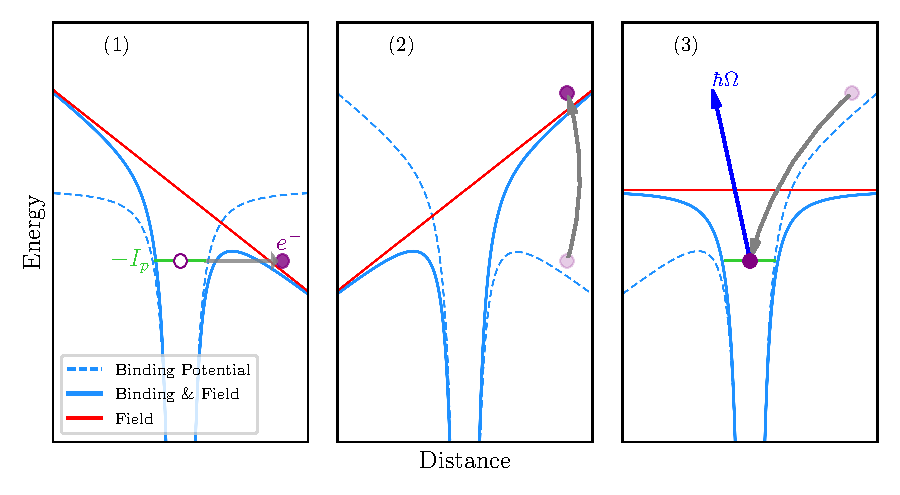
\includegraphics[width=1.0\textwidth]{figures/Introduction/3-step.pdf}
	\caption[Recollision model of high harmonic generation]{Recollision model of high harmonic generation.  The three steps are (1) tunnel ionization, (2) propagation/acceleration in the laser field, and (3) recombination and photoemission.}
	\label{fig:3-step}
\end{figure}

The mechanism behind this was not explained until 1993 by Schafer \textit{et al.} \cite{schaferThresholdIonizationHigh1993} in terms of an electron recollision process.  Shortly thereafter, Corkum's paper \cite{corkumPlasmaPerspectiveStrong1993} broke down this recollision process in terms of a simple three-step model consisting of ionization, propagation, and recombination.  The three steps in this model are shown schematically in figure \ref{fig:3-step}.  The first step in the three-step model is tunnel ionization where the strong laser field suppresses the atomic potential enough to allow the electron to tunnel through the potential energy barrier.  Once freed, the electron then undergoes the second step in the three-step process which is propagation in the field.  During this propagation, the electron picks up kinetic energy from the field and is driven back to the parent ion.  The maximum kinetic energy that can be gained from this process is approximately $3.17 U_p$, where the ponderomotive energy $U_p$ is given by
\begin{equation}
	U_p = \frac{e^2 \mathcal{E}_0^2}{4 m \omega_0^2}\propto I_0\lambda^2
\end{equation}
for a laser of wavelength $\lambda$ and peak intensity $I_0$.  Once the electron is driven back to the parent ion there are a few possible interaction pathways consisting of inelastic scattering, elastic scattering, and recombination.  The pathway of interest is recombination, and  when this occurs the excess energy picked up by the electron from the laser field is released in form of a photon of energy $\hbar\Omega$.  This means that the maximum photon energy that can be generated in this process (also known as the cutoff) is given by the relationship
\begin{equation}
	\hbar\Omega_{\mathrm{cutoff}} = I_p + 3.17 U_p,
\end{equation}
where $I_p$ is the ionization potential of the neutral atom.

\begin{figure}
	\centering
	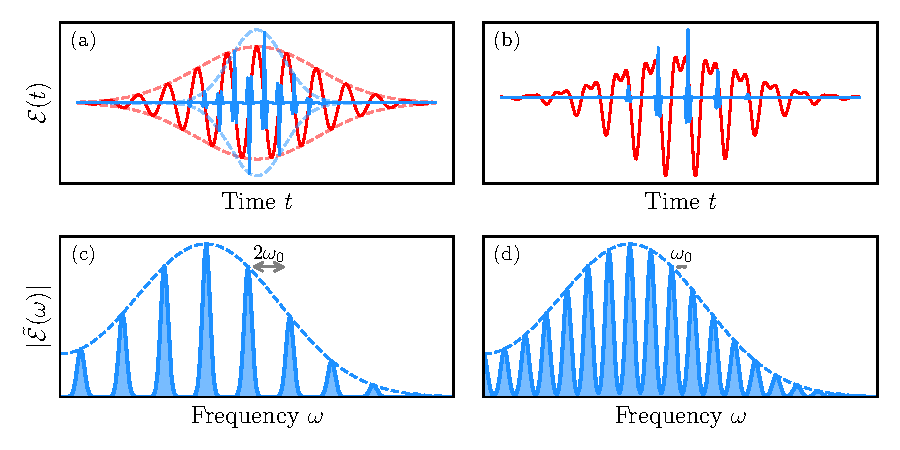
\includegraphics[width=1.0\textwidth]{figures/Introduction/time_to_freq.pdf}
	\caption[Example electric field of XUV APT and its frequency spectrum]{(a) Example of the electric field of an XUV APT.  There is a burst every half-cycle of the fundamental field period $\tau_0$.  (b)  Spectral amplitude of APT.  Harmonics are separated by $2\omega_0=4\pi/\tau_0$.  Bandwidth of each harmonic is determined by the number of cycles in the fundamental pulse, and the overall bandwidth is determined by the pulse duration of each burst in the train. (b) Example of a two-color $\omega-2\omega$ fundamental field.  The asymmetry of the pulse means there is a burst once every cycle. (d) The spectral amplitude for the asymmetric field, and now there are even and odd harmonics.  The dashed line in (c) and (d) represent the spectral amplitude of just one of the pulses in the pulse train.}
	\label{fig:time_to_freq}
\end{figure}

This three-step process repeats every half-cycle of the laser field, and as a consequence of this, the temporal structure of the generated XUV light is that of a ``train'' of short pulses every half-cycle of the fundamental field, as is shown in figure \ref{fig:time_to_freq}.  This structure is referred to as an attosecond pulse train (APT).  This structure was first experimentally measured in 2001 \cite{paulObservationTrainAttosecond2001} and showed that each burst in the APT has a pulse duration on the order of a few hundred attoseconds.  It is possible to isolate a single attosecond burst to create an isolated attosecond pulse (IAP), however this generally involves a single-cycle pulse \cite{hentschelAttosecondMetrology2001} or an engineered ellipticity across the pulse duration \cite{mashikoDoubleOpticalGating2008}.  These methods are not used in the experiments described herein, however there is another method that can modify the generated harmonic spectrum that will be used.  This method involves using a nonlinear crystal to generate the second harmonic of the fundamental, and when this pulse is temporally overlapped with the fundamental pulse it creates an asymmetric field, as shown in figure \ref{fig:time_to_freq}.  This asymmetric field means that there is now an attosecond burst only once per cycle of the fundamental.  The effect that this has on the spectrum is that there are now both even and odd harmonics.  When the bandwidth of each individual harmonic is large enough, then the harmonic comb can be treated like a pseudo-continuum of photon energies.  This idea of two-color generation can be extended to pulses with incommensurate frequencies to generate an IAP or harmonics of the beat frequency \cite{takahashiInfraredTwoColorMulticycle2010, haesslerEnhancedMulticolourGating2015}.



\section{Transient Absorption Spectroscopy}
\label{sec:intro_transient_absorption}

Now that the basics of high-harmonic generation has been laid out, the question becomes: What types of experiments can be performed with this unique light source?  Generally speaking, there are two main classes of experiments that can be performed.  One involves using the XUV APT to ionize a gas and collect photoelectrons, and the other involves measurement of the harmonic spectrum using a photon spectrometer.  Collecting photoelectrons allows for measurement such as RABBITT \cite{paulObservationTrainAttosecond2001} and streaking \cite{hentschelAttosecondMetrology2001} when an IR field is used to dress the gas that is being ionized  by the APT.  These techniques will not be used in any of the experiments described herein.  Instead, the harmonic spectrum will be measured using a photon spectrometer.  This gives access to the spectral amplitude of the XUV APT, and this enables transient absorption spectroscopy to be performed.

A schematic of how transient absorption spectroscopy works in gases is shown in figure \ref{fig:gas_TA_sketch}.  This is fundamentally a pump/probe measurement where an XUV APT serves as the pump and an IR pulses acts as the probe.  The idea is that the XUV pulse induces a polarization within the gas which decays on a timescale that is set by the lifetime of the excited state that the XUV populates.  When this time-domain picture is Fourier transformed through the measurement of the spectral amplitude, the absorption spectrum of the gas medium can be deduced.  This becomes transient absorption when an IR pulse is introduced at a variable time delay.  This IR pulse will perturb the induced polarization, and the resulting absorption spectrum will be modified.  This modification of the absorption spectrum as a function of time delay can be used to study the dynamics of the excited states within the gas.  This measurement is at the core of the work that was done in this dissertation, especially Chapters \ref{chap:ATS} and \ref{chap:CATS}, and more explicit details about transient absorption will be discussed in those Chapters.

\begin{figure}
	\centering
	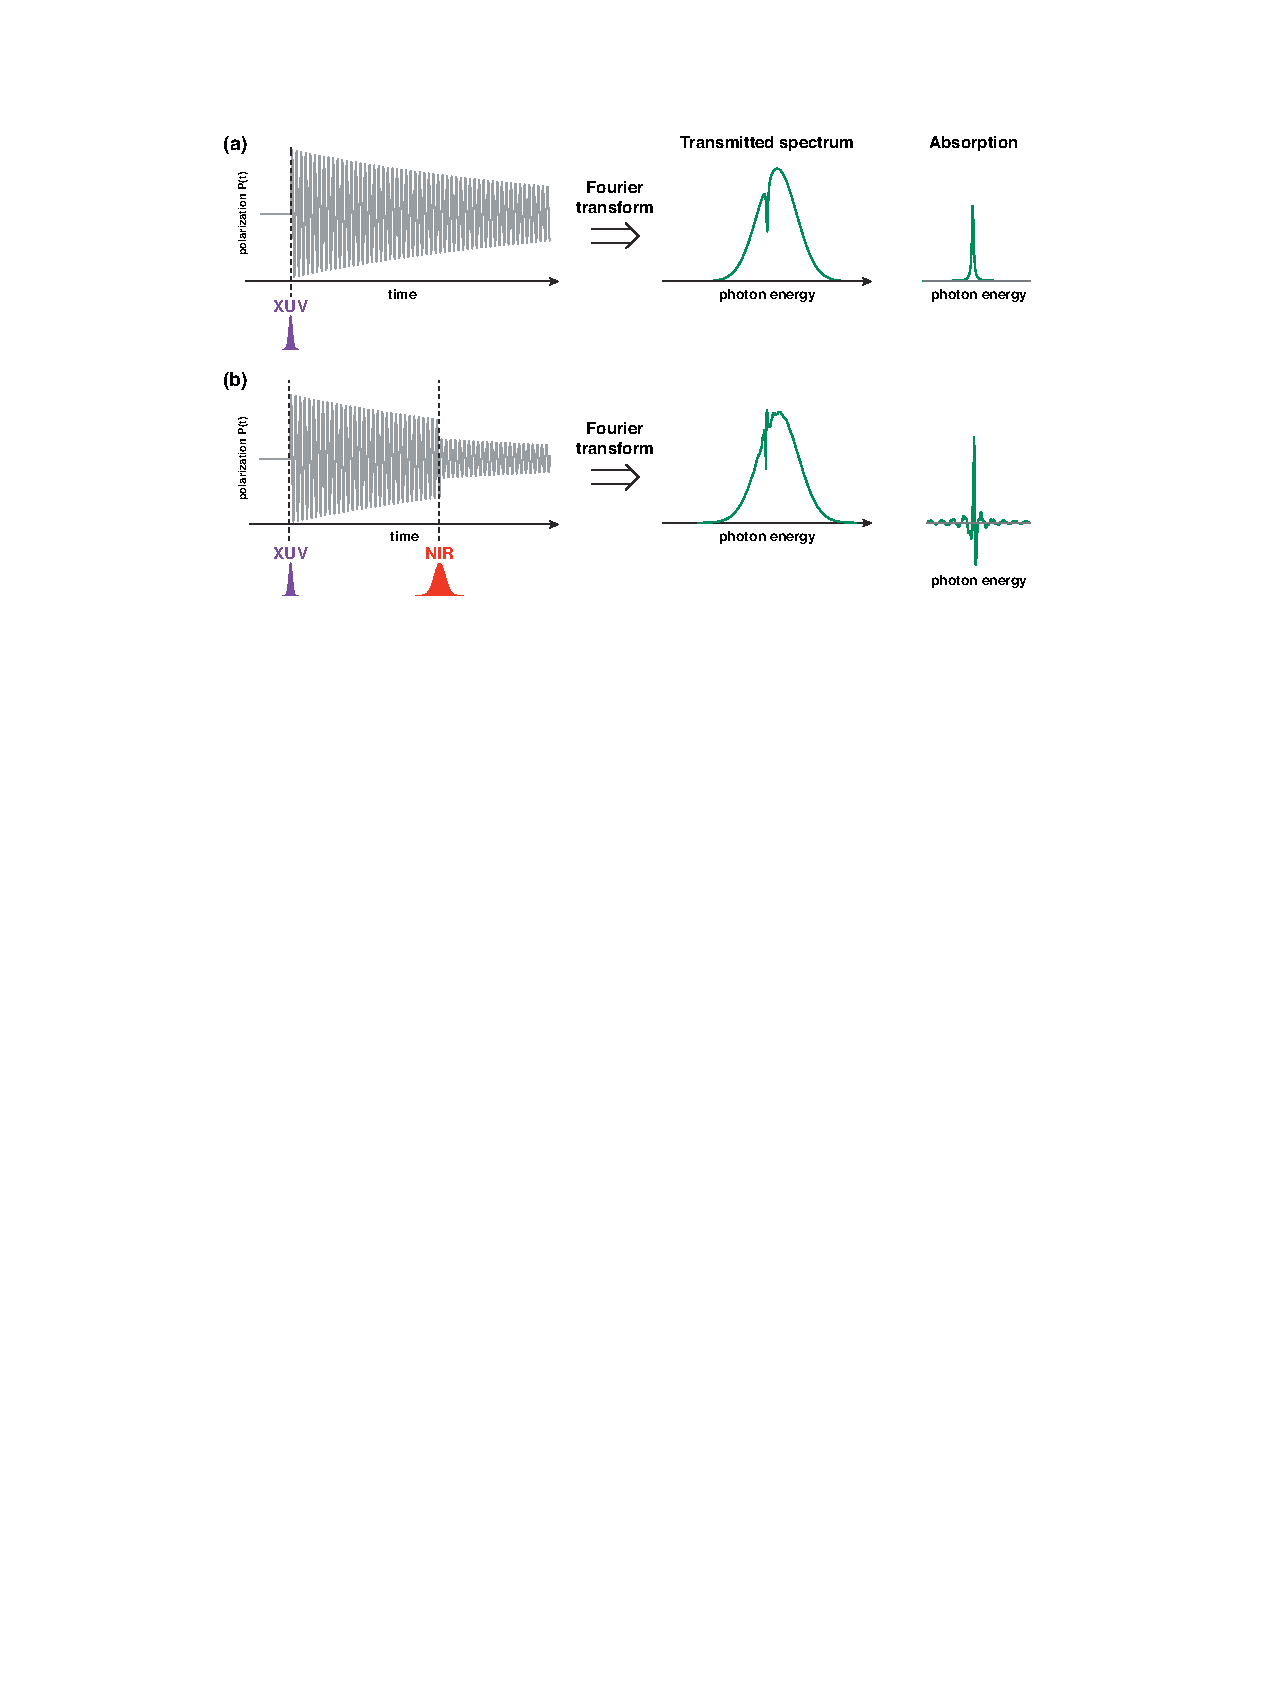
\includegraphics[width=1.0\textwidth]{figures/Introduction/gas_TA_sketch.pdf}
	\caption[Schematic of transient absorption in a gas]{(a) Simplified schematic of transient absorption in a gas.  In the time-domain, there is an induced polarization by the XUV APT that decays on a timescale set by the lifetime of the excited state.  The Fourier transform of this is the absorption spectrum.  (b) An IR pulse is introduced at a variable time delay that will perturb the polarization.  The modified absorption spectrum gives insight into the dynamics of the excited states of the gas.}
	\label{fig:gas_TA_sketch}
\end{figure}

